\documentclass[modern]{CORE-AAS/aastex631} 
%!! user commands }
%\usepackage{CORE-AAS/variables} 
\usepackage{datetime}
\usepackage[abs]{overpic}
\begin{document}

🚀

% The below puts a lightgrey "watermark" at top of manuscript to indicate compilation time. Comment out if not needed. 
\vspace*{-0.8cm}\noindent{\textcolor{lightgray}{Compiled: \currenttime\ \today\ (UTC)}

\title{\textbf{SAUNAS}: III. X-ray Scaling Relations of Diffuse Hot Gas Galactic Halos \footnote{Released on May, 11th, 2023}}
\author{Alejandro S. Borlaff}
\affiliation{Bay Area Environmental Research Institute, Moffett Field, CA 94035, USA}
\author{Pamela M. Marcum}
\affiliation{NASA Ames Research Center, Moffett Field, CA 94035, USA}

\begin{abstract}
Put the abstract here. 

\end{abstract}


\section{Background}
Here is the intro section \citep{aguerri+1998aj116_2136, bell+2006apj640_241,bell+2006apj652_270}. 

The first sentence in the intro! 

The second sentence in the intro \citep{erwin+2017mnras468_2058, falchi+2016an2_1600377}.

A 3rd sentence  in the background. 

%WIll this turn grey ?? 

\begin{figure*}[t!]
\begin{center}
 % trim left bottom right top 
 \begin{overpic}[trim={0 0 0 0}, clip, width=\textwidth]{NGC5084_6dF_spectra_comp.png}
\end{overpic}
\vspace{-0.5cm}
\caption
{Optical spectral energy distribution (SED) of NGC\,5084 as detected by the 6dF survey and the APO/DIS observations. \emph
{Top panel:} 4300-7000 \AA\ spectrum of the central 1.5 arcsec slit (APO/DIS, blue and red channels, in color) and the 6.7 arcsec radius fiber (6dF, black). \emph
{Bottom left:} Detail of the H$\gamma$ spectral range (4200 -- 4550 \AA), showing the core as detected by 6dF and APO/DIS, as well as the North, South, East, and West subregions avoiding the core. See the labels on each spectra. \emph
{Bottom right:} Same as previous for the 6400-6800 \AA (H$\alpha$) range. Vertical shadowed red lines represent the redshifted wavelengths of the typical absorption and emission lines in galaxies (H$\beta$, OIII, Mg, Na I, H$\alpha$), for reference.} 
\label{fig:NGC5084_optical_spectra}
\end{center}
\end{figure*}



Here is a comment, see if it changes color like it is supposed to. 
\subsection{Motivation}

The first sentence under motivation. \citep{bernardi+2006aj131_1288}

\subsection{more motivation}

second sentence under motivation.

Third sentence right here right NOW!! 

4th sentence 

5th sentence here 

\subsubsection{Goals}
First sentence in this section underneath Goals. 

\begin{figure*}[t!]
\begin{center}
 % trim left bottom right top 
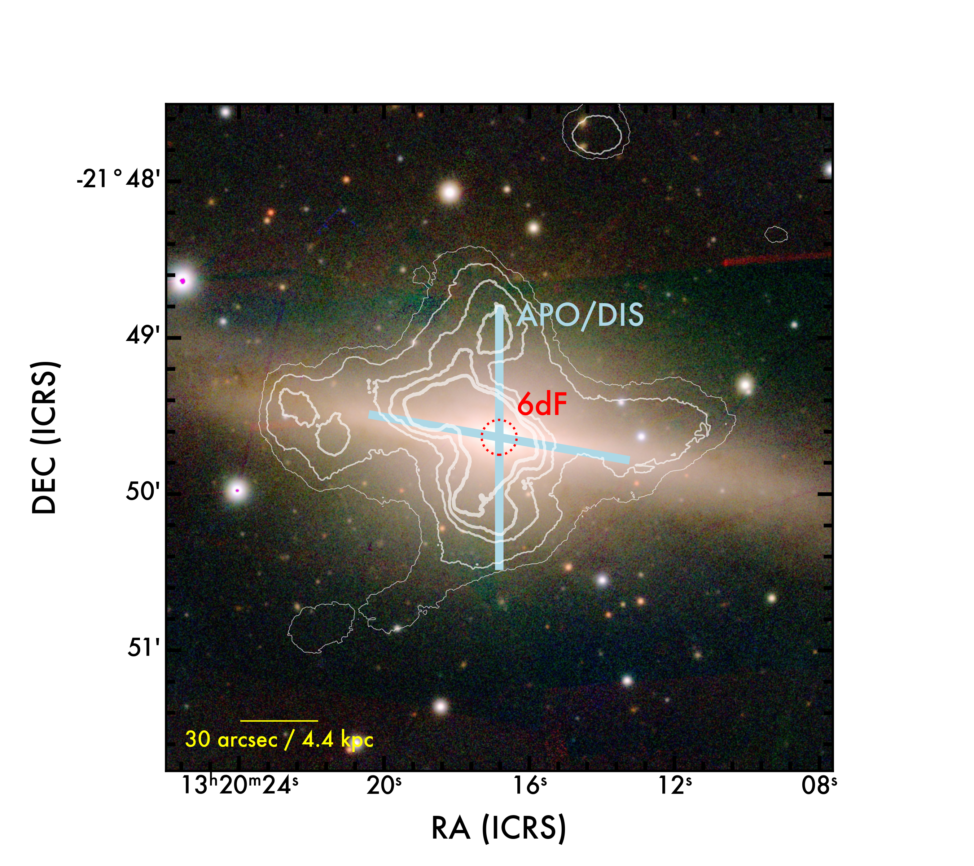
\includegraphics[trim={0 0 70 0}, clip, height=8.5cm]{NGC5084_spectra_regions_wide.png}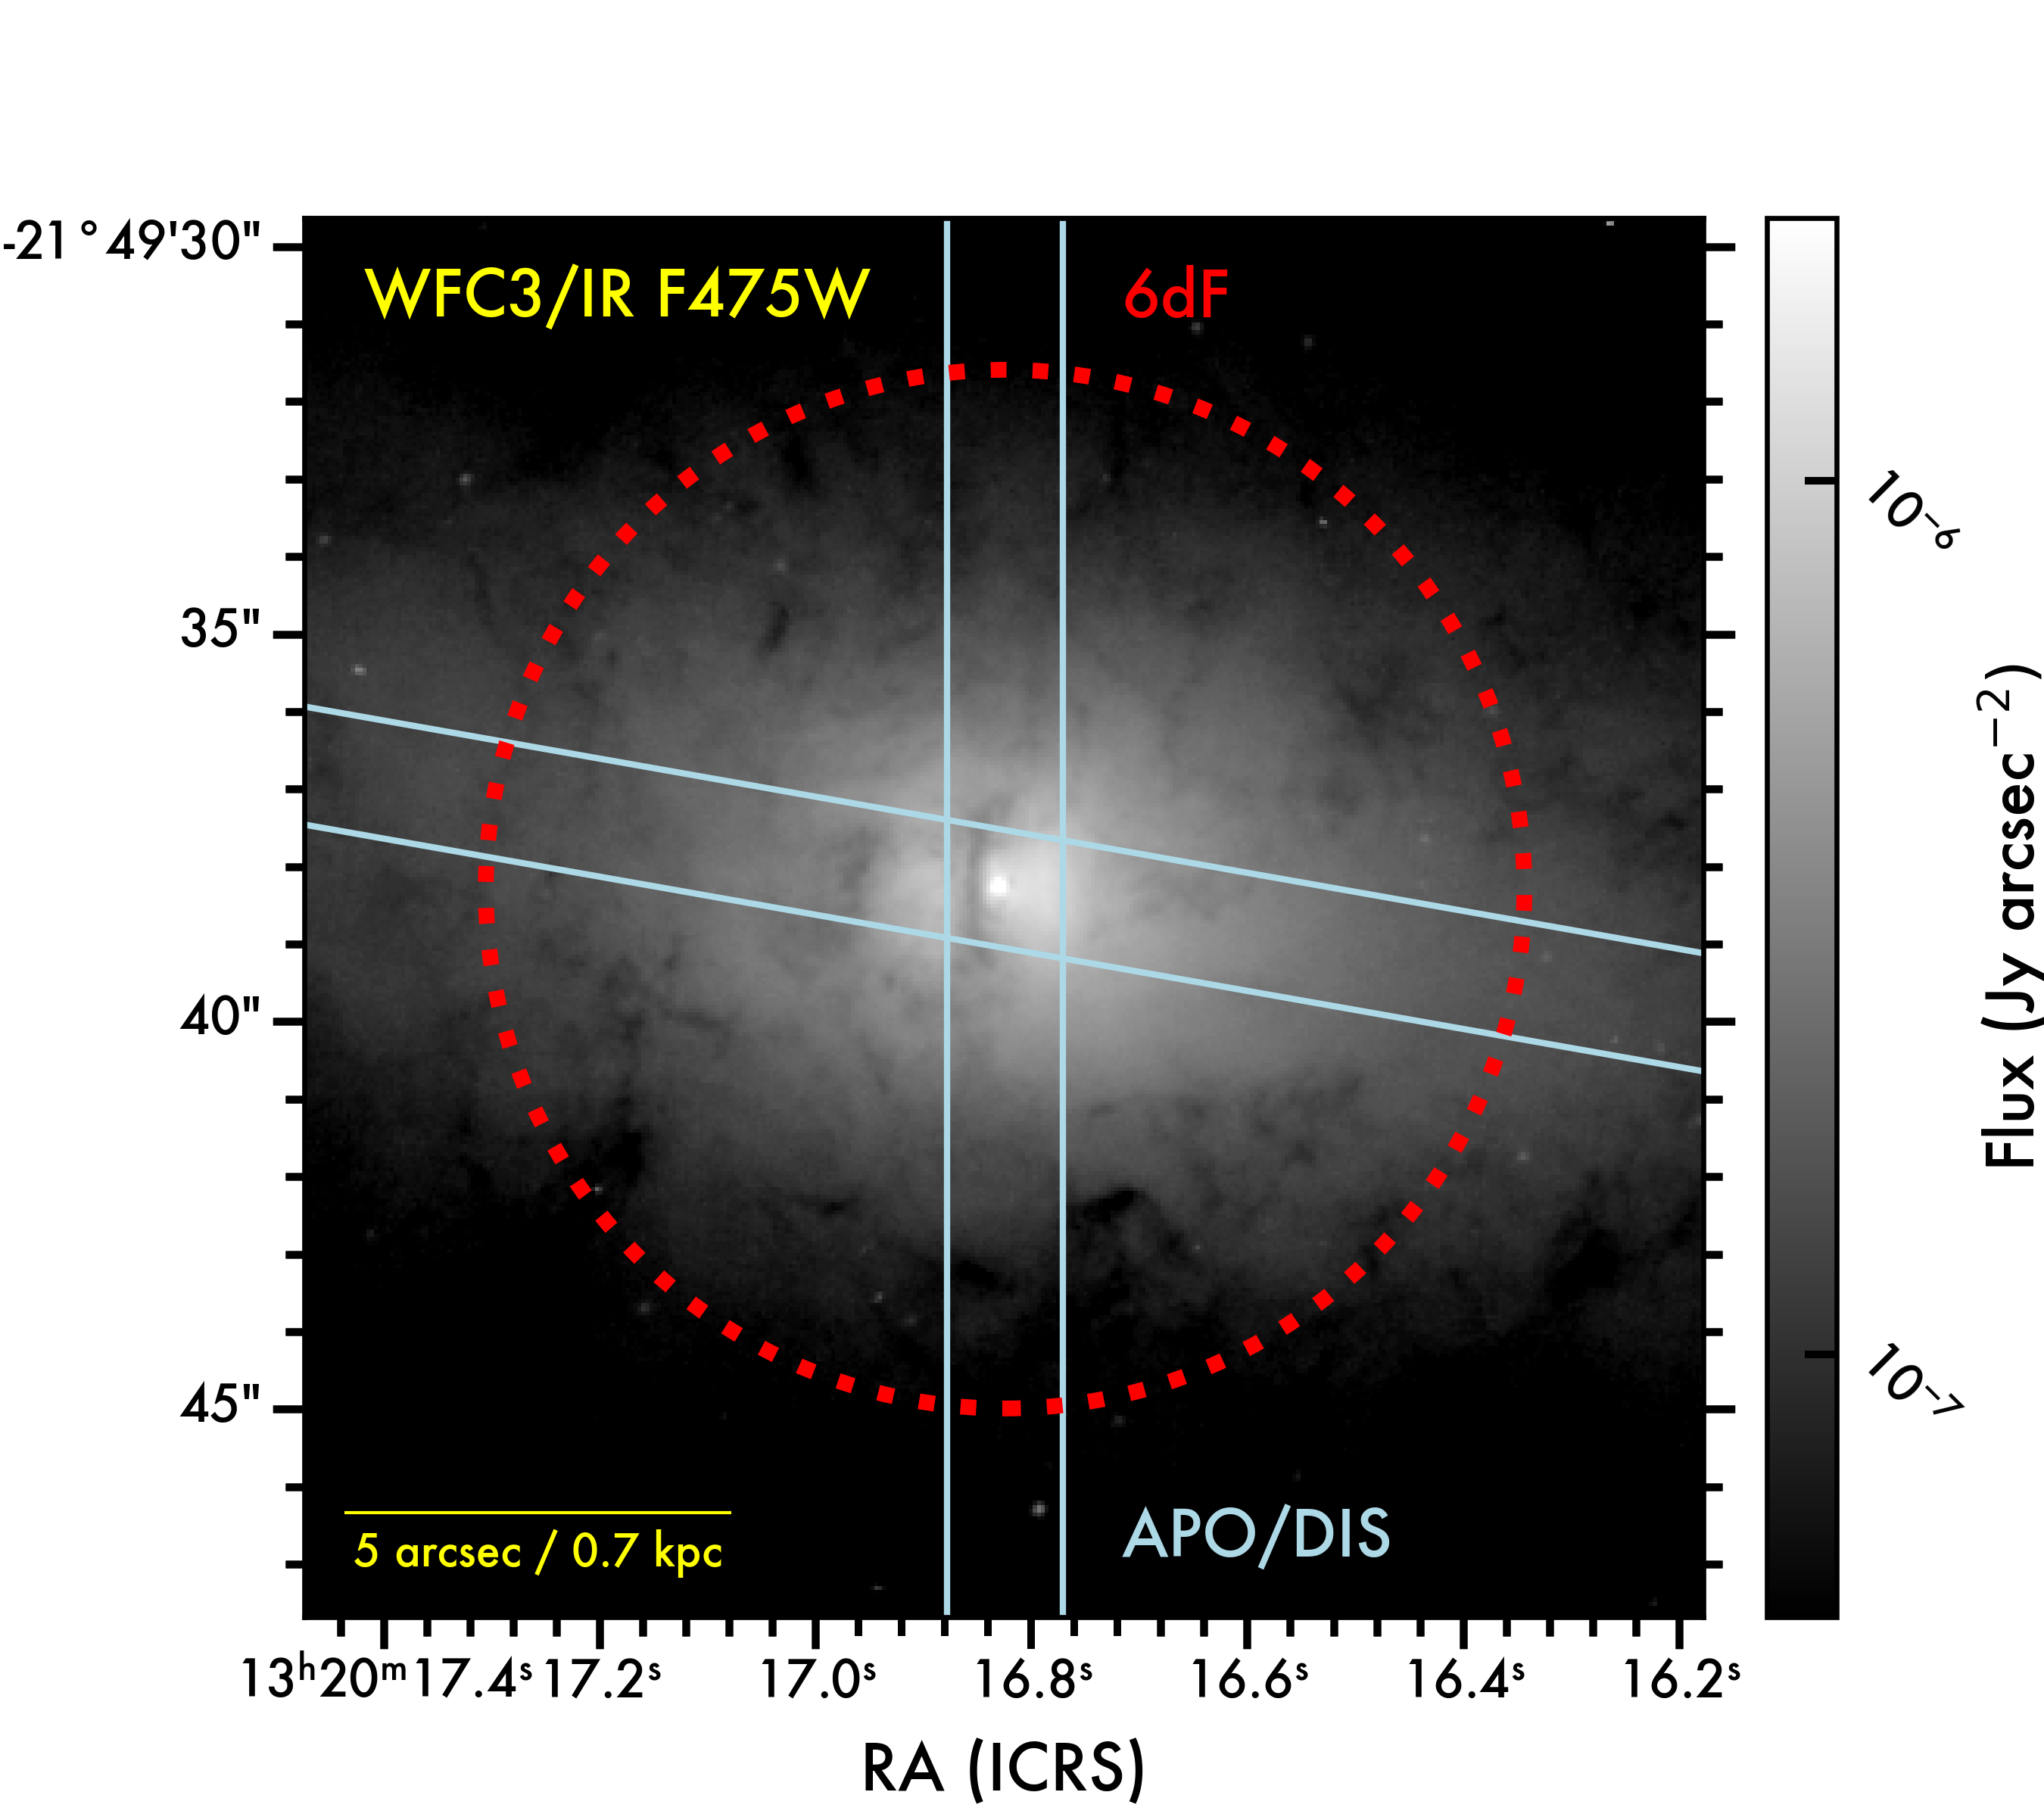
\includegraphics[trim={0 0 0 0}, clip, height=8.5cm]{NGC5084_regions_core.png}
\caption{Regions assigned for spectral analysis. \emph{Left panel:} White contours in the left panel represent the [2, 3, 5, 7, 10]$\sigma$ detection limits in the 0.3--2.0 keV band from Chandra/ACIS. The slit-shaped regions (1.5 arcsec wide) represent the APO/DIS optical spectra, defined to align with the major axis of the galaxy and the major axis of the circumnuclear disk. The circular core region, shown in the zoomed image, has a 3~arcsec radius. The RGB background image was generated using the $gri$ observations from Pan-STARRS. \emph{Right:} Close-up view of the core regions, showing the apertures for optical 6dF spectra ($R=3.4$ arcsec), and the APO/DIS slit-spectra. The background image represents the flux intensity in the F475W band from HST/WFPC2.} 
\label{fig:NGC5084_spectra_regions}
\end{center}
\end{figure*}


\section{Methods}
First sentence in methods section. 

\begin{acknowledgements}

\end{acknowledgements}
\vspace{5mm}
\facilities{Chandra} 

\software{CIAO, LIRA, VorBin} 

\bibliographystyle{CORE-AAS/aasjournal} 
\bibliography{Extragalactic}
\end{document} 


